\documentclass[12pt]{article}
\usepackage[utf8]{inputenc}

% Importing settings from setup.sty
\usepackage{setup}
\usepackage{booktabs}
\usepackage{multicol}
\usepackage{multirow}
\usepackage{glossaries}
\makenoidxglossaries

\newacronym{bof}{BOF}{Bag Of Features}
\newacronym{tfidf}{TF-IDF}{Term Frequency-Inverse Document Frequency}
\newacronym{sift}{SIFT}{Scale-Invariant Feature Transform}


\usepackage{tikz}
\usetikzlibrary{shapes.geometric, shapes.multipart, arrows, positioning}
\tikzstyle{data} = [ellipse, minimum width=1cm, minimum height=1.2cm,text centered, draw=black, fill=blue!20]
\tikzstyle{preprocessing_container} = [rectangle split,rectangle split parts=7, rectangle split draw splits=false, rounded corners, text width=8cm, minimum height=5cm, draw=black, fill=orange!20]
\tikzstyle{preprocessing} = [rectangle, rounded corners, minimum width=3cm, minimum height=1cm, draw=black, fill=orange!50]
\tikzstyle{dim_red} = [rectangle, rounded corners, minimum width=3cm, minimum height=1cm, draw=black, fill=brown!50]
\tikzstyle{classifier} = [rectangle, rounded corners, minimum width=3cm, minimum height=1cm, text centered, draw=black, fill=magenta!30]
\tikzstyle{result} = [rectangle, minimum width=3cm, minimum height=1cm, text centered, draw=black, fill=green!40]
\tikzstyle{arrow} = [thick,->,>=stealth]

% \pagenumbering{roman}
\begin{document}

% Inserting title page
\import{./}{title}

\pagenumbering{roman}
\tableofcontents
\listoffigures
\listoftables

\newgeometry{
    left=25mm,
    right=25mm,
    top=25mm,
    bottom=25mm}
\pagenumbering{arabic}

\section{Problem description}
The problem we are trying to solve consists of predicting whether an animal will be adopted from a shelter within 30 days, given several pieces of information on this animal. This problem is a clean and reduced version of a \href{https://www.kaggle.com/c/petfinder-adoption-prediction/overview}{Kaggle competition} dating back from 2019.

\section{Exploratory Data Analysis}
\label{sec: EDA}
We would like to get some basic information of the data set before diving into the machine learning solution. \\
The training set has shape \((8168 \times 16)\) and the test set has shape \((250 \times 16)\), where the column names and data types are summarized in Table \ref{table: column data type}. \\
\begin{table}[ht]
    \centering
    \begin{tabular}{ccccc}
        % \textbf{Type}                       &  & \multicolumn{1}{c}{\textbf{Column name}} \\ \midrule
        \toprule
        \multicolumn{2}{c}{\textsc{categorical}} & \textsc{numerical} & \textsc{text} & \textsc{image}          \\ \midrule
        Type                                     & MaturitySize       & Age           & Description    & Images \\
        Gender                                   & FurLength          & Fee                                     \\
        Breed                                    & Vaccinated                                                   \\
        Color1                                   & Dewormed                                                     \\
        Color2                                   & Sterilized                                                   \\
        Color3                                   & Health                                                       \\
        \bottomrule
    \end{tabular}
    \caption{Data types per column}
    \label{table: column data type}
\end{table} \\
Overall, the data set is very clean as it contains 0 NaN values.


\section{Problem Solution}
\subsection{Overview}
The problem can be solved by using a pipeling, which is represented in Figure \ref{fig: pipeline complete}. The pipeline consists of two steps:
\begin{itemize}
    \item Data Pre-processing
    \item Classification
\end{itemize}
We will detail these two steps in the following subsections.
\begin{figure}[ht]
    \centering
    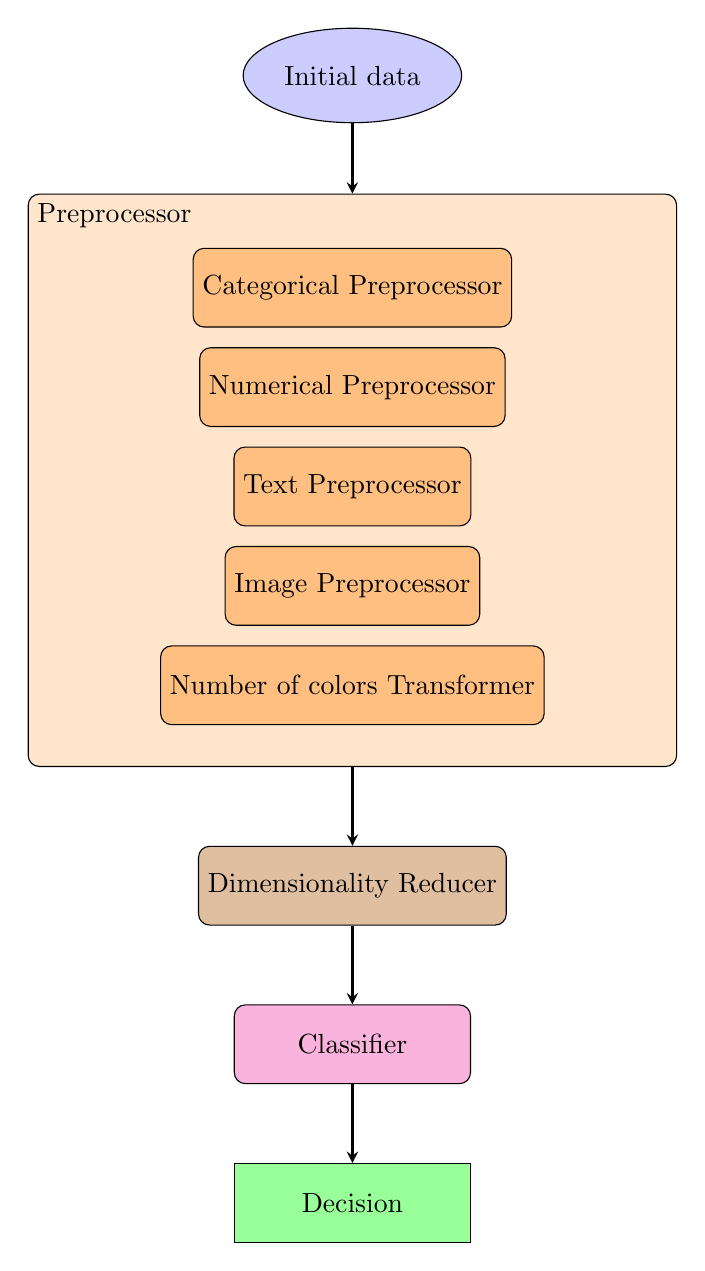
\begin{tikzpicture}[node distance=1.5cm]
        \node (start) [data] {Initial data};
        \node [align=center](preprocessing_container) [preprocessing_container, below of=start, anchor=north] {
            \nodepart[align=left]{one}Preprocessor
            \nodepart{two}
            \tikz{\node (categorical_preprocessor) [preprocessing] {Categorical Preprocessor}}
            \nodepart{three}
            \tikz{\node (numerical_preprocessor) [preprocessing] {Numerical Preprocessor}}
            \nodepart{four}
            \tikz{\node (text_preprocessor) [preprocessing] {Text Preprocessor}}
            \nodepart{five}
            \tikz{\node (image_preprocessor) [preprocessing] {Image Preprocessor}}
            \nodepart{six}
            \tikz{\node (nb_colors) [preprocessing] {Number of colors Transformer}}
        };
        \node (dim_red) [dim_red, below=1cm of preprocessing_container, anchor=north] {Dimensionality Reducer};
        \node (classifier) [classifier, below=1cm of dim_red, anchor=north] {Classifier};
        \node (result) [result, below=1cm of classifier, anchor=north] {Decision};

        \draw [arrow] (start) -- (preprocessing_container);
        \draw [arrow] (preprocessing_container) -- (dim_red);
        \draw [arrow] (dim_red) -- (classifier);
        \draw [arrow] (classifier) -- (result);
    \end{tikzpicture}
    \caption{Complete pipeline diagram}
    \label{fig: pipeline complete}
\end{figure}

\subsection{Data Preprocessing}
We saw in section \ref{sec: EDA} that the data is already fairly clean (\eg in terms of NA's). We still need to process the columns, which we do depending on the type of data they contain. As per Figure \ref{fig: pipeline complete}, we use:
\begin{itemize}
    \item A Categorical Preprocessor
    \item A Numerical Preprocessor
    \item A Text Preprocessor
    \item A Image Preprocessor
    \item A Transformer for the number of colors
\end{itemize}
We detail the above in their respective paragraphs.

\paragraph{Categorical Preprocessor} The Categorical Preprocessor is composed of a OneHotEncoder, which encodes categorical features as a one-hot numeric array. That is, for each of the categories, we create a new column with 1 if the initial column is of that category and 0 otherwise.

\paragraph{Numerical Preprocessor} The Numerical Preprocessor contains a StandardScaler. Its role is to center and scale each of the numerical variables in order to remove differences in orders of magnitude.

\paragraph{Text Preprocessor} The Text Preprocessor contains a TfidfVectorizer, which converts the raw comments from our text feature to a matrix of \gls{tfidf} features. We used a CountVectorizer initially, but it gave worse results than the \gls{tfidf}, which is why we kept the latter. The CountVectorizer counts the occurences of each word in the \textit{Description} column. A possible explaination of why the TfidfVectorizer performs better is that the features it produces not-only contain information about the frequency of each term, but they also account for the frequency of each word within the whole document.

\paragraph{Image Preprocessor} The Image Preprocessor consists of a custom  BOF\_extractor. It extracts \glspl{sift} and computes \gls{bof} on the images from the \textit{Images} column.

\paragraph{Number of colors Transformer} The Number of colors Transformer uses FunctionTransformer to compute how many colors the animal has (\ie colors different from ``Unknown''). It then sets the number of colors as a feature. \\
In addition to the preprocessors and transformers presented above, we perform Dimensionality Reduction:

\paragraph{Dimensionality Reducer} The Dimensionality Reducer consists of a TruncatedSVD transformer, which applies Latent Semantic Analysis to reduce the number of features in the data set.

\subsection{Classification}

\subsubsection{General approach}
Our approach for the Classification part separates in two parts
\begin{enumerate}
    \item Try various classifiers and evaluate their performance. Then, keep the best 5 classifiers.
    \item For the best 5 classifiers, fine-tune their hyperparameters and find the best one.
\end{enumerate}

\subsubsection{Select Models}
The algorithms tested are presented in Table \ref{table: all algorithms and accuracies}. We computed their accuracy following GridSearchCV (on the train data), then computed their prediction on the test data. We did not test XGBoost because it was too slow.

\begin{table}[H]
    \centering
    \begin{tabular}{ccc}
        \toprule
        \textsc{Classifier}        & \textsc{TestAccuracy} & \textsc{Train Accuracy} \\ \midrule
        RandomForestClassifier     & 0.592                 & 0.625                   \\
        BernoulliNB                & 0.584                 & 0.593                   \\
        GradientBoostingClassifier & 0.572                 & 0.633                   \\
        AdaBoostClassifier         & 0.572                 & 0.605                   \\
        MLPClassifier              & 0.564                 & 0.608                   \\
        GaussianNB                 & 0.552                 & 0.569                   \\
        GaussianProcessClassifier  & 0.548                 & 0.514                   \\
        SVC                        & 0.508                 & 0.525                   \\
        SGDClassifier              & 0.504                 & 0.516                   \\
        KNeighborsClassifier       & 0.496                 & 0.513                   \\
        DecisionTreeClassifier     & 0.476                 & 0.556                   \\
        \bottomrule
    \end{tabular}
    \caption{Accuracies on first prospect}
    \label{table: all algorithms and accuracies}
\end{table}

\subsubsection{Fine-tune hyperparameters}
As shown in Table \ref{table: all algorithms and accuracies}, the five best algorithms are GradientBoostingClassifier, RandomForestClassifier, AdaBoostClassifier, MLPClassifier and BernoulliNB. The next step is to select several hyperparameters for each of them and test them with GridSearchCV.
\begin{table}[ht]
    \centering
    \begin{tabular}{ccc}
        \toprule
        \textsc{Classifier}                         & \textsc{Hyperparameter} & \textsc{Values tested}                   \\
        \midrule
        \multirow{6}{*}{GradientBoostingClassifier} & learning\_rate          & 0.01, 0.02, 0.05, 0.1, 0.2               \\
                                                    & n\_estimators           & 50, 100, 150                             \\
                                                    & max\_depth              & 1, 3, 5                                  \\
                                                    & min\_samples\_split     & 1, 3, 5                                  \\
                                                    & min\_samples\_leaf      & 1, 2, 3                                  \\
                                                    & max\_features           & log2, sqrt                               \\
        \midrule
        \multirow{5}{*}{RandomForestClassifier}     & criterion               & gini, entropy                            \\
                                                    & max\_depth              & 100, 200, 300, 400, None                 \\
                                                    & min\_samples\_leaf      & 1, 2, 3, 4                               \\
                                                    & min\_samples\_split     & 8, 10, 12                                \\
                                                    & n\_estimators           & 60, 80, 100                              \\
        \midrule
        \multirow{3}{*}{AdaBoostClassifier}         & n\_estimators           & 10, 20, 30, 50, 70                       \\
                                                    & learning\_rate          & 0.5, 0.6, 0.7, 0.8, 1., 1.2              \\
                                                    & algorithm               & SAMME.R, SAMME                           \\
        \midrule
        \multirow{6}{*}{MLPClassifier}              & hidden\_layer\_sizes    & (50,100,50), (100,)                      \\
                                                    & learning\_rate          & constant, invscaling, adaptive           \\
                                                    & solver                  & adam                                     \\
                                                    & activation              & identity, logistic, tanh, relu           \\
                                                    & beta\_1                 & 0.8, 0.9, 0.99                           \\
                                                    & beta\_2                 & 0.99, 0.999, 0.9999                      \\
        \midrule
        \multirow{3}{*}{BernoulliNB}                & alpha                   & 0.01, 0.05, 0.1, 0.2, 0.3, 0.5, 1., 2.   \\
                                                    & binarize                & 0, 0.4, 0.5, 0.6, 0.65, 0.7, 0.8, 1., 2. \\
                                                    & fit\_prior              & True, False                              \\
        \bottomrule
    \end{tabular}
    \caption{Hyperparameters tested for the top 5 classifiers}
    \label{table: hyperparameters tested}
\end{table}

\section{Evaluation \& critical view}

\clearpage

\printnoidxglossaries

\end{document}